\section{Scopo e preparazione}

Si intende realizzare un'oscillatore sinusoidale a ponte di Wien con un OpAmp TL081
e osservarne il funzionamento, verificando le relazioni previste con le caratteristiche dei componenti utilizzati.
Si è dunque montato il circuito in \fig{circ}, utilizzato invariato in tutta l'esperienza; i valori misurati
per i componenti sono riportati in \tab{comp_mis}.

\begin{figure}[h]
	\centering
	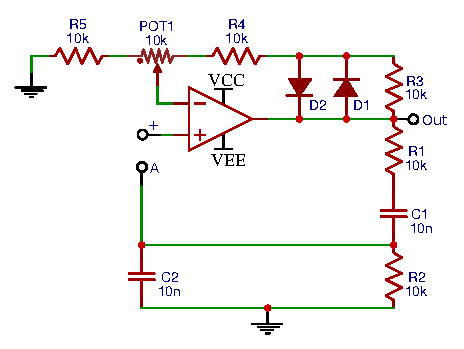
\includegraphics{circuito.pdf}
	\caption{Circuito oscillatore a ponte di Wien.}
	\label{f:circ}
\end{figure}

\begin{table}[h]
	\centering
	\begin{tabular}{ *{5}{S[table-figures-decimal=2]} *{2}{S[table-figures-decimal=1, table-figures-uncertainty=1]} }
		{$R_1$ [\si{\kohm}]} & {$R_2$ [\si{\kohm}]}	& {$R_3$ [\si{\kohm}]} & {$R_4$ [\si{\kohm}]} & {$R_5$ [\si{\kohm}]}
			& {$C_1$ [\si{\nano\farad}]} & {$C_2$ [\si{\nano\farad}]} \\
		\midrule
		9.95(9) & 9.94(9) & 9.90(9) & 9.94(9) & 9.90(9) & 10.8(5) & 10.1(4) \\
	\end{tabular}
	\caption{Misure dei componenti.}
	\label{t:comp_mis}
\end{table}

La sezione superiore del circuito, costituita dai diodi, dal potenziometro e dalle resistenze $R_{3-4-5}$,
è la rete di feedback necessaria ad utilizzare l'OpAmp come amplificatore (non invertente) rispetto all'ingresso non invertente,
mentre la sezione inferiore, costituita dal parallelo e dalla serie di resistenza e condensatore, realizza il feedback di Wien
che, riportato all'ingresso non invertente dell'OpAmp, rende il circuito un oscillatore (a patto che sia verificata la condizione di Barkhausen).

\section{Loop gain}

Intendiamo innanzitutto misuare il guadagno della rete di feedback di Wien: abbiamo dunque collegato l'ingresso
non invertente dell'OpAmp al generatore d'onda e inviato un sengale sinusoidale di ampiezza picco-picco $\approx \SI{500}{\mV}$
a varie frequenze comprese tra \SIrange[range-phrase = \text{ e }]{500}{3000}{\Hz},
misurando il segnale in uscita al punto A del circuito.

% TODO: spiegare i dati e fittare! perché betaA con fase di pi??
